\begin{exercise}
      {ID-51caed6448753cf4de9bf791661089e31e3c6b27}
      {Augensumme}
  \ifproblem\problem
    Wie groß ist die Wahrscheinlichkeit, mit zwei Würfeln die Augensumme 5
    zu würfeln?
  \fi
  %\ifoutline\outline
  %\fi
  \ifoutcome\outcome
    \begin{center}
      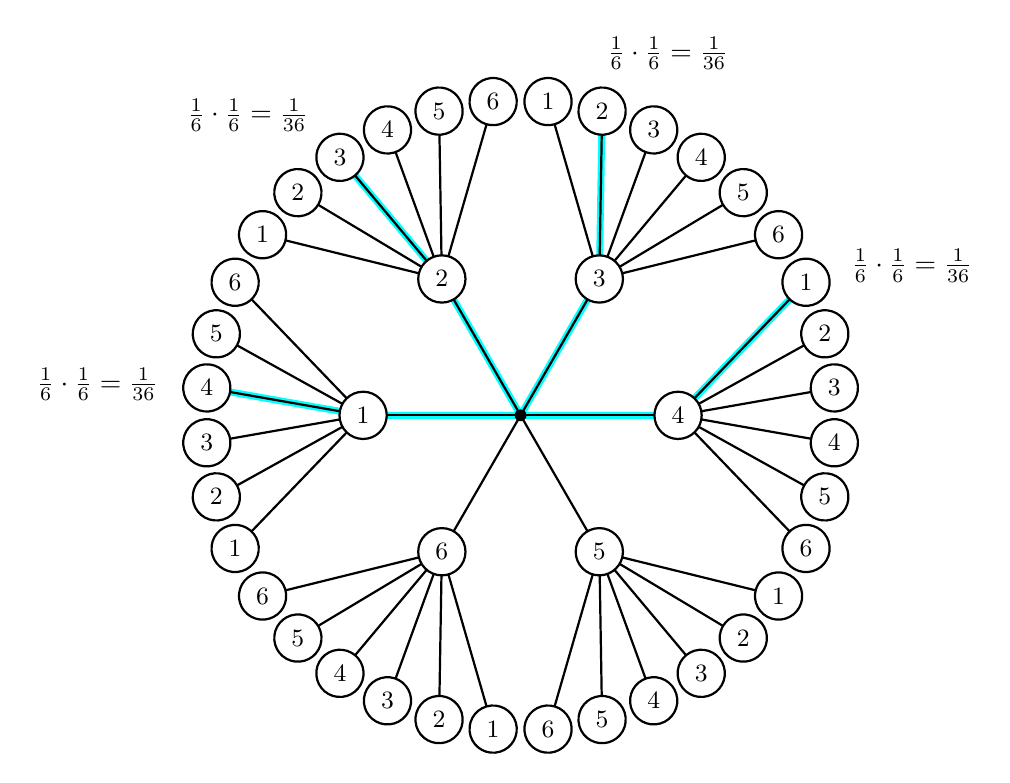
\begin{tikzpicture}
        % Markierungen
        \begin{scope}[line width=2.5pt, draw=Cyan]
          \draw (0, 0) -- (180:2cm) -- (175:4cm);
          \draw (0, 0) -- (120:2cm) -- (125:4cm);
          \draw (0, 0) -- ( 60:2cm) -- ( 75:4cm);
          \draw (0, 0) -- (  0:2cm) -- ( 25:4cm);
        \end{scope}
        \node[right] at (25:4.5cm) {$\frac{1}{6}\cdot\frac{1}{6}=\frac{1}{36}$};
        \node[right] at (78:4.7cm) {$\frac{1}{6}\cdot\frac{1}{6}=\frac{1}{36}$};
        \node[left] at (124:4.6cm) {$\frac{1}{6}\cdot\frac{1}{6}=\frac{1}{36}$};
        \node[left] at (175:4.5cm) {$\frac{1}{6}\cdot\frac{1}{6}=\frac{1}{36}$};
        % Kanten
        \begin{scope}[line width=0.8pt]
          \draw (0, 0) -- (  0:2cm);
          \draw (0, 0) -- ( 60:2cm);
          \draw (0, 0) -- (120:2cm);
          \draw (0, 0) -- (180:2cm);
          \draw (0, 0) -- (240:2cm);
          \draw (0, 0) -- (300:2cm);
        \end{scope}
        \begin{scope}[line width=0.8pt]
          \draw (0:2cm) -- ( 25:4cm);
          \draw (0:2cm) -- ( 15:4cm);
          \draw (0:2cm) -- (  5:4cm);
          \draw (0:2cm) -- (355:4cm);
          \draw (0:2cm) -- (345:4cm);
          \draw (0:2cm) -- (335:4cm);
        \end{scope}
        \begin{scope}[line width=0.8pt, rotate=60]
          \draw (0:2cm) -- ( 25:4cm);
          \draw (0:2cm) -- ( 15:4cm);
          \draw (0:2cm) -- (  5:4cm);
          \draw (0:2cm) -- (355:4cm);
          \draw (0:2cm) -- (345:4cm);
          \draw (0:2cm) -- (335:4cm);
        \end{scope}
        \begin{scope}[line width=0.8pt, rotate=120]
          \draw (0:2cm) -- ( 25:4cm);
          \draw (0:2cm) -- ( 15:4cm);
          \draw (0:2cm) -- (  5:4cm);
          \draw (0:2cm) -- (355:4cm);
          \draw (0:2cm) -- (345:4cm);
          \draw (0:2cm) -- (335:4cm);
        \end{scope}
        \begin{scope}[line width=0.8pt, rotate=180]
          \draw (0:2cm) -- ( 25:4cm);
          \draw (0:2cm) -- ( 15:4cm);
          \draw (0:2cm) -- (  5:4cm);
          \draw (0:2cm) -- (355:4cm);
          \draw (0:2cm) -- (345:4cm);
          \draw (0:2cm) -- (335:4cm);
        \end{scope}
        \begin{scope}[line width=0.8pt, rotate=240]
          \draw (0:2cm) -- ( 25:4cm);
          \draw (0:2cm) -- ( 15:4cm);
          \draw (0:2cm) -- (  5:4cm);
          \draw (0:2cm) -- (355:4cm);
          \draw (0:2cm) -- (345:4cm);
          \draw (0:2cm) -- (335:4cm);
        \end{scope}
        \begin{scope}[line width=0.8pt, rotate=300]
          \draw (0:2cm) -- ( 25:4cm);
          \draw (0:2cm) -- ( 15:4cm);
          \draw (0:2cm) -- (  5:4cm);
          \draw (0:2cm) -- (355:4cm);
          \draw (0:2cm) -- (345:4cm);
          \draw (0:2cm) -- (335:4cm);
        \end{scope}
        % Start
        \fill (0, 0) circle[radius=0.75mm];
        % 1. Ebene
        \filldraw[fill=white, draw=black, line width=0.8pt] (  0:2cm) circle[radius=3mm] node{{\small4}};
        \filldraw[fill=white, draw=black, line width=0.8pt] ( 60:2cm) circle[radius=3mm] node{{\small3}};
        \filldraw[fill=white, draw=black, line width=0.8pt] (120:2cm) circle[radius=3mm] node{{\small2}};
        \filldraw[fill=white, draw=black, line width=0.8pt] (180:2cm) circle[radius=3mm] node{{\small1}};
        \filldraw[fill=white, draw=black, line width=0.8pt] (240:2cm) circle[radius=3mm] node{{\small6}};
        \filldraw[fill=white, draw=black, line width=0.8pt] (300:2cm) circle[radius=3mm] node{{\small5}};
        % 2. Ebene
        \begin{scope}[rotate=5]
          \filldraw[fill=white, draw=black, line width=0.8pt] (  30:4cm) circle[radius=3mm] node{{\small6}};
          \filldraw[fill=white, draw=black, line width=0.8pt] (  40:4cm) circle[radius=3mm] node{{\small5}};
          \filldraw[fill=white, draw=black, line width=0.8pt] (  50:4cm) circle[radius=3mm] node{{\small4}};
          \filldraw[fill=white, draw=black, line width=0.8pt] (  60:4cm) circle[radius=3mm] node{{\small3}};
          \filldraw[fill=white, draw=black, line width=0.8pt] (  70:4cm) circle[radius=3mm] node{{\small2}};
          \filldraw[fill=white, draw=black, line width=0.8pt] (  80:4cm) circle[radius=3mm] node{{\small1}};
          \filldraw[fill=white, draw=black, line width=0.8pt] (  90:4cm) circle[radius=3mm] node{{\small6}};
          \filldraw[fill=white, draw=black, line width=0.8pt] ( 100:4cm) circle[radius=3mm] node{{\small5}};
          \filldraw[fill=white, draw=black, line width=0.8pt] ( 110:4cm) circle[radius=3mm] node{{\small4}};
          \filldraw[fill=white, draw=black, line width=0.8pt] ( 120:4cm) circle[radius=3mm] node{{\small3}};
          \filldraw[fill=white, draw=black, line width=0.8pt] ( 130:4cm) circle[radius=3mm] node{{\small2}};
          \filldraw[fill=white, draw=black, line width=0.8pt] ( 140:4cm) circle[radius=3mm] node{{\small1}};
          \filldraw[fill=white, draw=black, line width=0.8pt] ( 150:4cm) circle[radius=3mm] node{{\small6}};
          \filldraw[fill=white, draw=black, line width=0.8pt] ( 160:4cm) circle[radius=3mm] node{{\small5}};
          \filldraw[fill=white, draw=black, line width=0.8pt] ( 170:4cm) circle[radius=3mm] node{{\small4}};
          \filldraw[fill=white, draw=black, line width=0.8pt] ( 180:4cm) circle[radius=3mm] node{{\small3}};
          \filldraw[fill=white, draw=black, line width=0.8pt] ( 190:4cm) circle[radius=3mm] node{{\small2}};
          \filldraw[fill=white, draw=black, line width=0.8pt] ( 200:4cm) circle[radius=3mm] node{{\small1}};
          \filldraw[fill=white, draw=black, line width=0.8pt] ( 210:4cm) circle[radius=3mm] node{{\small6}};
          \filldraw[fill=white, draw=black, line width=0.8pt] ( 220:4cm) circle[radius=3mm] node{{\small5}};
          \filldraw[fill=white, draw=black, line width=0.8pt] ( 230:4cm) circle[radius=3mm] node{{\small4}};
          \filldraw[fill=white, draw=black, line width=0.8pt] ( 240:4cm) circle[radius=3mm] node{{\small3}};
          \filldraw[fill=white, draw=black, line width=0.8pt] ( 250:4cm) circle[radius=3mm] node{{\small2}};
          \filldraw[fill=white, draw=black, line width=0.8pt] ( 260:4cm) circle[radius=3mm] node{{\small1}};
          \filldraw[fill=white, draw=black, line width=0.8pt] ( 270:4cm) circle[radius=3mm] node{{\small6}};
          \filldraw[fill=white, draw=black, line width=0.8pt] ( 280:4cm) circle[radius=3mm] node{{\small5}};
          \filldraw[fill=white, draw=black, line width=0.8pt] ( 290:4cm) circle[radius=3mm] node{{\small4}};
          \filldraw[fill=white, draw=black, line width=0.8pt] ( 300:4cm) circle[radius=3mm] node{{\small3}};
          \filldraw[fill=white, draw=black, line width=0.8pt] ( 310:4cm) circle[radius=3mm] node{{\small2}};
          \filldraw[fill=white, draw=black, line width=0.8pt] ( 320:4cm) circle[radius=3mm] node{{\small1}};
          \filldraw[fill=white, draw=black, line width=0.8pt] ( 330:4cm) circle[radius=3mm] node{{\small6}};
          \filldraw[fill=white, draw=black, line width=0.8pt] ( 340:4cm) circle[radius=3mm] node{{\small5}};
          \filldraw[fill=white, draw=black, line width=0.8pt] ( 350:4cm) circle[radius=3mm] node{{\small4}};
          \filldraw[fill=white, draw=black, line width=0.8pt] (   0:4cm) circle[radius=3mm] node{{\small3}};
          \filldraw[fill=white, draw=black, line width=0.8pt] (  10:4cm) circle[radius=3mm] node{{\small2}};
          \filldraw[fill=white, draw=black, line width=0.8pt] (  20:4cm) circle[radius=3mm] node{{\small1}};
        \end{scope}
      \end{tikzpicture}
    \end{center}
    \begin{equation*}
      P(\text{\glqq Augensumme 5\grqq})=\frac{1}{36}+\frac{1}{36}+\frac{1}{36}+\frac{1}{36}=\frac{4}{36}=\frac{1}{9}\approx11\,\text{\%}
    \end{equation*}
  \fi
\end{exercise}
